\section{Introduction}
LLM agents increasingly need to learn from and plan within complex environments. This makes \emph{world models}, which support hypothetical rollouts under candidate actions, increasingly important. They matter for two reasons. First, agentic reinforcement learning relies on experience-driven scaling, where world models can generate simulated experience to improve learning efficiency \cite{ha2018recurrent,georgievpwm}. Second, LLM agents are expected to operate over long horizons, where delayed consequences and compounding uncertainty make reliable reasoning difficult; world models let agents simulate downstream effects before acting, supporting more consistent decisions \cite{hao2023reasoning,gu2024your}. In novel settings, however, these models cannot always be pre-built and must be synthesized or adapted on demand.

%%%%%%%%%%% 引入我们需要 discrete-event executable world model

A growing body of work has explored world models across domains \cite{genie3,feng2025web}, but much of it focuses on environments governed by physical dynamics or spatial structure, such as robotic control, visual navigation, and interactive 3D worlds. In contrast, many high-impact real-world systems, including supply chains, procurement networks, service operations, and business processes, are governed by discrete interactions among multiple entities. In these settings, outcomes depend less on continuous physical evolution than on the ordering, timing, and causal dependencies of events. Improving agent performance therefore requires models that capture process structure at the system level, where interventions can yield gains beyond localized physical or spatial optimization \cite{mckinsey2019automation,mgi2021iot,gvr2025process}.

This motivates the study of \emph{discrete-event world models}: models that represent macro-level environments through state transitions, logical rules, and structured event traces.
% Currently, obtaining world models for these systems often falls toward one of two ends of a spectrum. 
More broadly, existing methods to constructing world models tend to fall near one of two extremes. 
At one end, \emph{hand-engineered simulators} explicitly encode environment dynamics through domain rules and process logic. Although reproducible and interpretable, they require substantial human effort and are difficult to adapt online. 
At the other end, \emph{implicit neural approaches} learn to predict future states directly \cite{hao2023reasoning,li2025word}. 
Although flexible, they are vulnerable to long-horizon inconsistency.
In discrete, process-driven domains, such drift can manifest as invalid event sequences, violated resource constraints, or inconsistent entity states, making purely implicit methods difficult to rely on for consequential planning. Therefore, a valuable middle ground remains underdeveloped: world models that are simultaneously long-horizon consistent, behaviorally verifiable, and synthesizable on demand. 

We study this middle ground by formulating world-model construction as the synthesis of executable discrete-event simulators from natural-language environment specifications. The specification provides the domain entities, events, timing assumptions, and causal dependencies, while the generated simulator provides an explicit operational model for rolling out candidate actions. Because the model is executable code, its state updates, event scheduling, and transition logic can be reproduced, inspected, and verified against domain constraints. This preserves the consistency of explicit simulation while reducing the adaptation burden of hand-engineered simulators.


% 介绍我们关心的问题的主要问题
%  (引入 LLM 的面条代码与试错成本痛点)
This raises two key challenges. First, realistic environments are structurally complex. Single-pass generation often fails because one localized error can invalidate the full system. Iterative coding agents can compensate through trial-and-error debugging, but those loops incur high token costs and latency, making them unattractive for on-demand synthesis. Second, evaluation is difficult because natural-language specifications are inherently underspecified. One specification may admit multiple valid simulators with different internal abstractions and edge-case behavior. Code-level equivalence is therefore ill-posed, while aggregate KPIs are too coarse: similar KPIs can arise from incorrect event logic, and different KPIs can arise from equally valid interpretations.

% 引入devs作为生成脚手架来解决第一个问题
% 修改：解释何为模块化，并且进一步提高devs特性和我们的pipeline的关联度。
To address the first challenge, we adopt the Discrete Event System Specification (DEVS) formalism \cite{zeigler2000theory,RiscoMartin2023xDEVS} as the structural scaffold for simulator construction. DEVS prevents logical entanglement by requiring components to interact only through explicit ports. Building on this isolation, we introduce \methodname{}, a DEVS model generation pipeline that first plans the system hierarchy and port interfaces, and then synthesizes component logic under these interaction contracts. This decomposition bounds context, enables parallel generation, and avoids costly global debugging loops.

% 引入我们构造的benchmark来解决第二个问题
To address the second challenge, we introduce a benchmark based on \emph{trace-based conformance}: evaluating whether the observable behavior of a generated simulator satisfies the temporal, causal, and semantic constraints implied by the specification. Rather than assuming a single canonical implementation, we derive evaluation tasks from high-quality open-source DEVS models whose dynamics provide structured behavioral constraints. The benchmark measures two quantities: \emph{operational success}, which captures whether a simulator respects the required I/O contract and trace schema, and \emph{behavioral conformance}, which captures whether its traces satisfy the expected micro-level state transitions and macro-level causal dependencies. These criteria provide a stable, fine-grained assessment of simulator correctness.

Together, these elements yield a specification-driven framework for generating and rigorously evaluating discrete-event world models. Across seven benchmark scenarios and four model families, our experiments demonstrate two primary advantages:
(i), \methodname{} exhibits highly predictable efficiency scaling. While iterative agents hit a vertical wall of non-terminating debugging cycles on complex tasks, our decoupled pipeline reliably translates computation time into continuous task completion, scaling to near 100\% generation success rate. 
(ii), ablations reveal a critical architectural trade-off: directly enforcing strict DEVS rules imposes a severe cognitive penalty on LLMs. However, \methodname{} successfully absorbs this burden through its explicit planning phase (\plantree{}), ultimately surpassing the performance of easy-to-write, unconstrained monolithic baselines. 

Beyond evaluation, the resulting model hierarchy, port interfaces, and standardized trace schema provide reusable structure for downstream applications. As a proof of concept, we show that automated tools can parse the DEVS topology as a blueprint to systematically instantiate Godot graphical assets, driving real-time frontend animations purely from backend event traces. More broadly, this work supports hybrid systems in which LLMs act as decision-making entities inside event-driven simulators, enabling complex multi-agent processes to be specified, simulated, and inspected from natural-language descriptions \cite{bergemann2026training}.

\begin{figure*}[t]
\centering
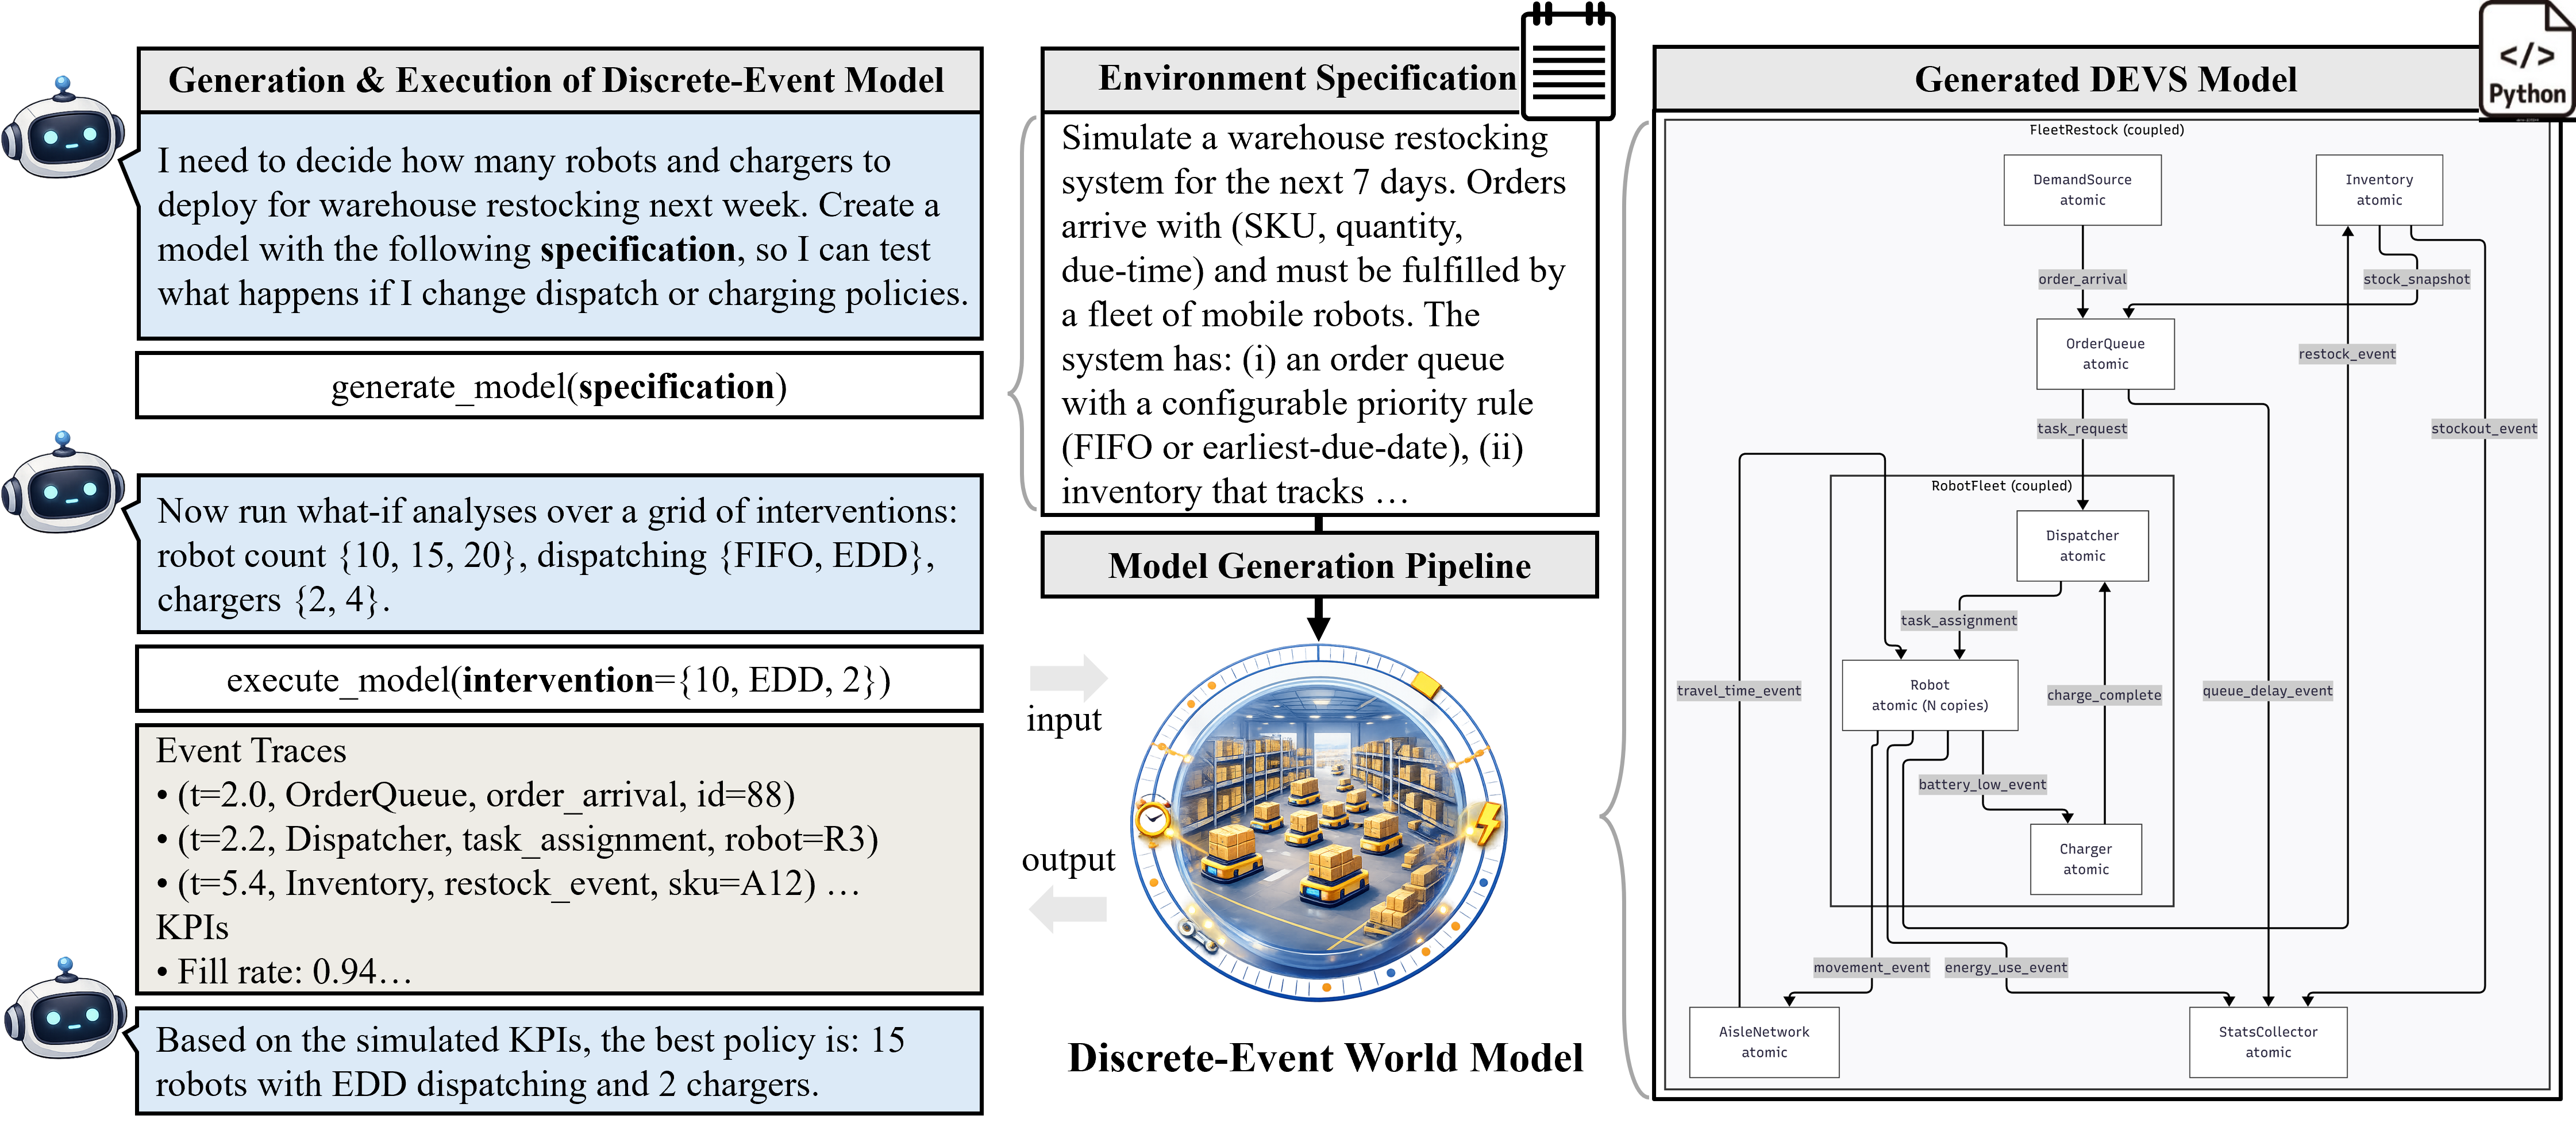
\includegraphics[width=0.99\textwidth]{imgs/complete_pipeline.png}
\caption{Illustrative example of the generation and execution of a discrete-event world model for a warehouse robot fleet restocking task.
To facilitate planning, a natural-language specification is translated into a world model, which exposes a standardized execution interface for interventions (e.g., fleet size, dispatching rule, charger count) and emits a structured event trace and performance metrics. We propose to operationalize such a world model as a DEVS model composed of interacting atomic and coupled components, each representing an entity with local state, event-handling logic, and timing semantics. Interactions among entities are realized through event messages routed via component ports, while event timing is governed by component-specific time-advance and transition functions. This enables systematic what-if analysis and comparative evaluation for online planning.}
\label{fig:complete_pipeline}
\end{figure*}